\chapter{Transformer：整体结构、训练目标与内部组件}
\label{chap:transformer}

\begin{keybox}[先看整台模型，再看一层内部]
Transformer 把一组 token 向量变成一组包含上下文信息的向量。注意力负责位置之间的信息交换，前馈网络负责位置内部的特征变换，残差连接与归一化让这些层可以反复堆叠。网络最后接什么输出头、每个位置允许读取什么信息，以及用什么损失训练，共同决定它是文本表示模型、条件生成模型还是自回归语言模型。
\end{keybox}

在展开具体结构之前，先回答一个容易被跳过的问题：离散文本的生成，为什么最后是自回归占了主流？这里没有一条定理保证它，只是几件事叠在一起的结果。

第一，链式法则给出的是精确、逐项归一化的似然。每个位置只是一个 \(|\mathcal V|\) 类分类问题，损失是交叉熵，训练目标没有额外的近似。第二，teacher forcing 让所有位置在一次前向里并行监督，而且每个 token 都贡献一项损失，监督信号密集。第三，序列长度是可变的，生成长度由模型自己决定，不需要为不同长度设计特殊机制。第四，条件化几乎免费：提示词就是前缀，条件生成不需要另外的接口。第五，工程上键值缓存（Key--Value cache，KV cache）把串行解码的重复计算去掉，批处理与推测解码再把固定开销摊薄，串行不再等于不可接受。

离散扩散是主要的替代方案。它需要额外设计吸收态和转移矩阵，多个位置同时去掩码时还要保证联合分布的一致性；连续扩散在图像上的成功不能直接搬过来。它在并行采样和可控性上有优势，但训练目标和采样程序都比自回归复杂。

所以更准确的说法是：自回归在离散序列上的优势，来自“目标简单、监督密集、工程成熟”的叠加。如果硬件形态或算法改变——例如并行采样的收益变得更大，或者离散扩散的训练目标变得更简单——这个格局未必不变。

\section{Transformer 的共同骨架与三种模型结构}

\subsection{共同输入与层内骨架：从 token 到上下文表示}

在自然语言处理中，原始文字先由分词器（tokenizer）按预先确定的规则转换为 token 编号序列 \(x_1,\ldots,x_T\)，每个编号都属于有限词表 \(\mathcal V\)。token 可以是完整单词、字、子词、标点或其他文本片段；词表通常还包含 BOS、EOS 等特殊 token。编号只是类别标签，编号顺序只是词表中的索引，与语义距离无关。词表和切分规则通常在模型训练前确定，它们会影响序列长度 \(T\) 和后续词表矩阵的大小。

分词器本身是一个独立的预处理算法。以字节对编码（Byte-Pair Encoding，BPE）为例：从字符或字节开始，统计语料中相邻符号对的频率，反复把最高频的一对合并成新符号，直到词表达到预定大小；合并规则固定后，训练和推理都使用同一套规则~\cite{sennrich2016bpe,radford2019gpt2}。字节级 BPE 先把文本转成 UTF-8 字节，因此任何字符都能表示：未登录词只会拆成更多的字节 token，词表中不需要未知词标记 UNK（unknown）。

词表大小是一个取舍。词表越大，同样的文本切成越少的 token，序列更短，注意力和 KV cache 的成本随之下降；但输入嵌入和输出 softmax 的参数量、以及稀有 token 的统计量都会增加。中文、日文等多字节文字在字节级词表下通常占更多 token；数字常被拆成单个数字，这对算术有利也有弊；科学文本里的公式、单位和上下标往往没有专门的 token，会被切成不自然的片段。这些切分方式直接影响模型看到什么。

特殊 token 还承担结构标记：BOS、EOS、填充、对话角色等。对话模板把多轮消息拼成一条带标记的序列，训练和推理必须使用同一套模板，否则条件分布会对不上。不同 tokenizer 的 per-token 概率不能直接比较，这一点在评价语言模型时会再次用到。

输入嵌入矩阵 \(E\in\R^{|\mathcal V|\times d}\) 为每个 token 存一条 \(d\) 维可训练向量。第 \(t\) 个编号通过查表得到 \(e_t=E_{x_t,:}^{\mathsf T}\)；这等价于用该编号的 one-hot 向量选中矩阵的一行，实现时无需显式构造 one-hot。word2vec 的基本想法也是从语境学习词向量；它学到的同一个词的向量通常不随句子改变~\cite{mikolov2013efficient}。Transformer 同样从查表向量开始，再加上位置信息，通过注意力让每个位置从允许读取的其他位置收集信息，形成随上下文变化的表示 \(h_t\)；输入矩阵 \(E\) 通常直接由模型的训练损失更新，无需先训练一个独立的 word2vec 模型。

例如，假设词表把 \texttt{bank} 作为一个 token，“the river bank”和“a local bank”中的 \texttt{bank} 都从 \(E\) 取同一初始向量，但上下文表示可以分别指向“河岸”和“银行”。双向 Encoder 中，一个位置可利用整句；GPT（Generative Pre-trained Transformer，生成式预训练 Transformer）的因果层只能利用当前位置及此前的前缀，不能提前读取后面的词。图 \ref{fig:token-to-context} 把“固定的查表向量变成随语境变化的向量”画成一条输入路径。

\begin{figure}[H]
\centering
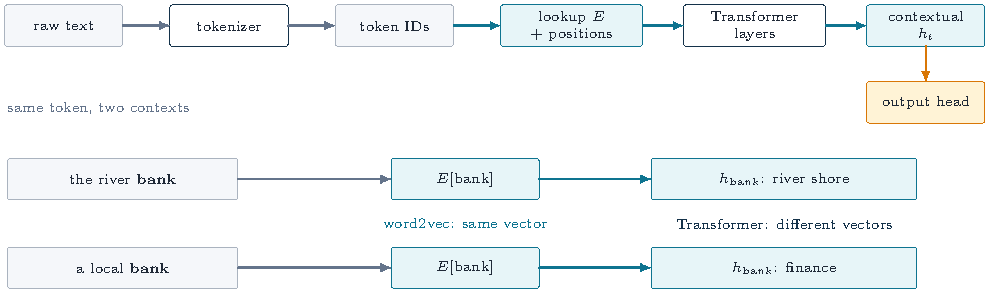
\includegraphics[width=\textwidth]{token_to_context.pdf}
\caption{自然语言输入到 Transformer 表示的路径。分词器把文字映射到词表编号，嵌入矩阵为编号提供初始向量；示例假设 \texttt{bank} 是一个 token，两句话查到相同的初始向量，经过上下文信息交换后得到不同的表示。输出头再把表示用于词表预测或具体任务。}
\label{fig:token-to-context}
\end{figure}

最早的 Transformer 用于机器翻译，采用编码器与解码器（Encoder--Decoder）两部分：先把完整源句编码，再根据源句表示逐步生成译文~\cite{vaswani2017attention}。后来广泛使用的两条路线是 BERT 主要使用编码器学习文本表示~\cite{devlin2019bert}；以及 GPT，使用只有因果解码层的网络学习序列生成~\cite{radford2018gpt}。图 \ref{fig:transformer-overview} 展示三种结构的信息流。

三条路线共享上述输入路径和层内骨架。\textbf{自注意力}让一个位置从可见的其他位置读取信息；\textbf{前馈网络}（Feed-Forward Network，FFN）在每个位置内部变换通道；\textbf{残差连接}把子层输出加回输入，归一化控制数值尺度。多层堆叠后，每个位置得到包含内容与上下文的表示。网络最后可以把这些表示投影到词表并做 softmax，以预测 token，也可以接分类等任务输出头。

\begin{figure}[H]
\centering
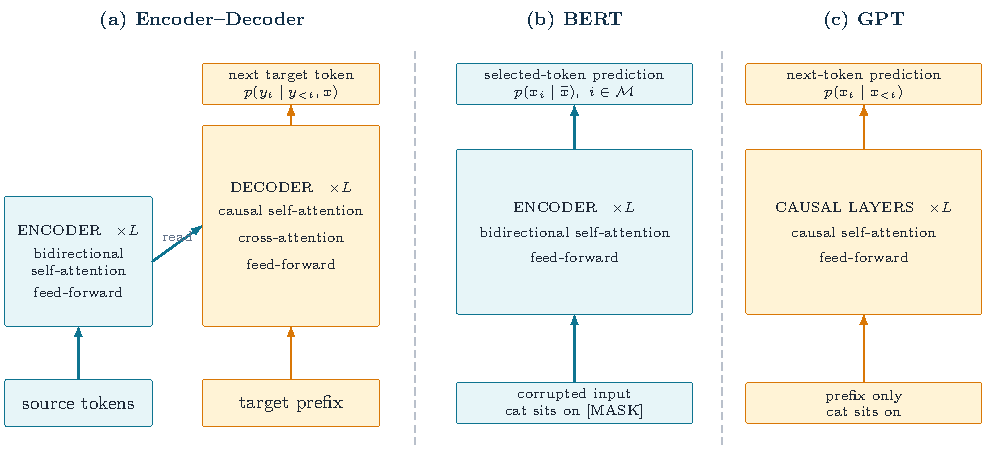
\includegraphics[width=\textwidth]{transformer_overview.pdf}
\caption{Transformer 的三种整体结构，箭头表示信息流。(a) 原始编码器读取完整源序列，解码器读取目标前缀，并通过交叉注意力访问源表示；(b) BERT 对经过遮盖或扰动的输入做双向编码，预测被选位置的原词；(c) GPT 只读取因果前缀，逐位置预测下一个 token。每个层框内部还包含残差连接与归一化。遮盖输入内容与限制注意力可见范围是两种不同操作。}
\label{fig:transformer-overview}
\end{figure}

\subsection{原始 Encoder--Decoder：先读源句，再写目标句}

设源句为 \(x_{1:S}\)，目标译文为 \(y_{1:T}\)。Encoder 的每一层包含双向自注意力和 FFN：源句已经完整给定，所以任意源位置都能读取其他源位置。堆叠后得到 \(H^{\mathrm{src}}=\operatorname{Encoder}(x_{1:S})\)，它是每个源位置的上下文表示。

Decoder 的每一层有三个子层：先用因果自注意力读取已经给定的目标前缀，再用\textbf{交叉注意力}读取 \(H^{\mathrm{src}}\)，最后经过 FFN。自注意力在“当前译文内部”交换信息，交叉注意力在“译文与源句之间”交换信息：当前译文表示决定要查找什么，编码器输出提供可查询的内容。因此解码器既知道自己写到哪里，也能随时回看源句。

词表投影与 softmax 把解码器输出变成条件概率，整台模型学习
\begin{equation}
 p_\theta(y_{1:T}\mid x_{1:S})
 =\prod_{t=1}^{T}p_\theta(y_t\mid y_{<t},x_{1:S}),\qquad
 \mathcal L_{\mathrm{translation}}
 =-\E_{(x,y)}\sum_{t=1}^{T}\log p_\theta(y_t\mid y_{<t},x_{1:S}).
 \label{eq:encoder-decoder-loss}
\end{equation}
训练时把真实目标序列右移一位送入 Decoder，使用 teacher forcing；因果遮罩使所有目标位置可以并行计算，却无法读取各自的正确答案。推理时先编码一次源句，再由解码器从 BOS 开始逐 token 生成，直到 EOS。这个结构适合“完整输入已经给定、输出需要依次产生”的条件生成任务。

\subsection{BERT：双向编码与遮盖词预测}
\label{sec:bert-mlm-link}

如果目标是分类、检索、句子匹配或抽取答案，通常希望一个词的表示同时利用左右两侧上下文。BERT 因此使用双向 Encoder。比如“他坐在河流的岸边”，后面的“河流”有助于确定前面相关词的含义；这种信息在整段文字已给定的任务中完全可用。

预训练又需要让这些表示从无标注文本中学到东西。若把原句完整输入，再要求每个位置输出它自己，模型很容易仅复制输入。遮盖语言建模（Masked Language Modeling，MLM）选择一部分位置集合 \(\mathcal M\)，将这些位置的输入遮盖或扰动，得到 \(\widetilde x\)，再让模型恢复原始 token：
\begin{equation}
 \mathcal L_{\mathrm{MLM}}
 =-\E_{x,\mathcal M,\widetilde x}\sum_{i\in\mathcal M}
 \log p_\theta(x_i\mid\widetilde x).
 \label{eq:bert-mlm}
\end{equation}
MLM 的损失只在被选中的位置计算。原始 BERT 的扰动机制除了替换为 \texttt{[MASK]}，也包括替换为随机 token 或保留原 token；因此“被选中预测的位置”与“实际显示 \texttt{[MASK]} 的位置”不必完全相同。例如输入“猫坐在 \texttt{[MASK]} 上”，目标是“垫子”，网络可以同时利用空缺两侧的信息；这就是完形填空目标与双向可见范围的配合。

原始 BERT 还加入下一句预测这一辅助任务：用分类汇总 token（Classification token，CLS）的表示判断两个句段是否在原文中相邻。若标签 \(b\in\{0,1\}\)，预测相邻的概率为 \(r_\theta\)，损失为
\begin{equation}
 \mathcal L_{\mathrm{sentence}}=-\E[b\log r_\theta+(1-b)\log(1-r_\theta)],\qquad
 \mathcal L_{\mathrm{BERT}}=\mathcal L_{\mathrm{MLM}}+\mathcal L_{\mathrm{sentence}}.
\end{equation}
这里的“下一句预测”是句段关系二分类；它不生成下一句。后续编码器模型可修改或去掉该辅助任务。预训练完成后，可以把 CLS 表示接分类头，或把各 token 表示接标注与答案位置预测头，再用具体任务的损失微调。

BERT 的填空条件分布利用了空缺左右的信息，MLM 因而没有直接给出从左到右的联合概率分解。若要生成一整段新文本，还需要另外设计填空顺序或迭代生成程序；第 \ref{sec:discrete-diffusion} 节的掩码扩散给出一种逐步恢复程序。下面 GPT 的目标则直接规定了从左到右的采样程序。

\subsection{GPT：因果解码与下一 token 预测}

GPT 采用 Decoder-only 结构。它保留因果自注意力、FFN、残差和归一化，并省去原始 Decoder 中读取独立 Encoder 输出的交叉注意力。提示词与生成结果放在同一条序列里，后面的位置只允许读取前面已经给出的内容。名称中的“Decoder”在这里描述这种因果序列结构，无需另配一个 Encoder。

考虑“猫、坐、在、垫子、上”这条序列。训练输入与标签错开一个位置：
\begin{equation}
 \begin{array}{c|cccccc}
 \text{输入}&\mathrm{BOS}&\text{猫}&\text{坐}&\text{在}&\text{垫子}&\text{上}\\
 \text{目标}&\text{猫}&\text{坐}&\text{在}&\text{垫子}&\text{上}&\mathrm{EOS}
 \end{array}.
\end{equation}
输入“在”的位置可以读取此前的“猫、坐”和当前“在”，预测下一个 token“垫子”。因果遮罩阻止它读取后面的“垫子”，所以标签不会通过注意力泄漏。所有位置都能同时产生这种预测，训练损失就是第 \ref{sec:autoregressive} 节的自回归 NLL：
\begin{equation}
 \mathcal L_{\mathrm{GPT}}=-\E_x\sum_{t=1}^{T}\log p_\theta(x_t\mid x_{<t}),\qquad
 p_\theta(x_{1:T})=\prod_{t=1}^{T}p_\theta(x_t\mid x_{<t}).
 \label{eq:gpt-next-token}
\end{equation}
预测“下一个词”更准确地说是预测下一个 token，它可能是完整词，也可能是子词或标点。这个目标直接来自联合概率的链式分解；生成时先采一个 token，再将其追加到前缀，重复使用同一个模型即可得到整段文本。GPT 系列的通用文本预训练沿用这一目标；指令微调通常只在回答部分计算相同的逐 token 损失，偏好优化与奖励训练则会增加或替换训练目标，第 \ref{chap:training-methods} 章再展开。

\subsection{结构、可见范围与训练损失的对应}

Encoder 和 Decoder 的层内骨架很相似，都使用自注意力、FFN、残差连接和归一化。就\textbf{自注意力的可见范围}而言，Encoder 中每个 token 可以读取所有输入 token；Decoder 的自注意力加上 causal mask（因果掩码），第 \(t\) 个位置只能读取自己和此前的 token。原始 Encoder--Decoder 架构中的 Decoder 还通过交叉注意力读取 Encoder 的输出。

BERT 做完形填空，是为了在双向上下文中学习恢复被扰动的内容；GPT 预测下一 token，是为了让训练时的条件与逐步生成时可得到的前缀一致。两者常用的逐位置损失都是词表上的交叉熵，区别主要在条件里能看到什么，以及在哪些位置计算损失。原始 Encoder--Decoder 也预测下一目标 token，但额外以完整源序列为条件（表 \ref{tab:transformer-objectives}）。

\begin{table}[ht]
\centering\small
\begin{tabularx}{\textwidth}{>{\bfseries}p{25mm} X X X}
\toprule
结构 & 当前预测可读取什么 & 典型预训练/训练目标 & 整台模型的用途\\
\midrule
Encoder--Decoder & 完整源序列与目标前缀 & 目标序列的条件 NLL & 翻译等序列到序列生成\\
BERT & 扰动后输入的左右上下文 & 被选位置的 MLM；原始版本另有句段关系损失 & 上下文表示与任务微调\\
GPT & 当前目标之前的 token & 各目标位置的下一 token NLL & 从前缀逐步生成新序列\\
\bottomrule
\end{tabularx}
\caption{三种结构的差别先体现在信息可见性与监督目标，内部都复用注意力和前馈网络。}
\label{tab:transformer-objectives}
\end{table}

接下来沿 GPT 使用的因果解码层展开内部组件。图 \ref{fig:transformer-overview} 中的一层由注意力、FFN、残差和归一化组成：注意力决定从哪些位置读取，位置编码补充顺序信息，FFN 组合通道特征，残差与归一化支持深层堆叠。

\section{查询、键、值与因果 mask}

给定序列表示矩阵 \(X\in\R^{T\times d}\)，其中 \(T\) 是本次送入模型的 token 数（序列长度），\(d\) 是每个 token 在残差流中的模型维度。单头投影通常把它映射到 \(Q,K\in\R^{T\times d_k}\) 和 \(V\in\R^{T\times d_v}\)；多头实现中常取 \(d_k=d_v=d/h\)，\(h\) 为 query head 数。这里的查询（Query，Q）、键（Key，K）和值（Value，V）分别表示“想找什么”“按什么匹配”和“读取什么”。于是
\begin{equation}
 Q=XW_Q,\quad K=XW_K,\quad V=XW_V,
\end{equation}
投影矩阵由训练学习。给定投影后的三个矩阵，单头注意力定义为
\begin{equation}
 \mathrm{Attn}(Q,K,V)=\softmax\left(\frac{QK^\top}{\sqrt{d_k}}+M\right)V,
\end{equation}
其中未来位置在 \(M\) 中设为 \(-\infty\)；以 \(X\) 为输入时，先用上式计算 \(Q,K,V\)，再代入 \(\mathrm{Attn}(Q,K,V)\)。

多头注意力（Multi-Head Attention，MHA）把上面这一步在各组投影上重复 \(h\) 次，再把结果拼回模型维度：
\begin{equation}
 \mathrm{head}_i=\mathrm{Attn}(XW_{Q,i},XW_{K,i},XW_{V,i}),\qquad
 \mathrm{MHA}(X)=\operatorname{Concat}(\mathrm{head}_1,\ldots,\mathrm{head}_h)W_O.
\end{equation}
这里 \(W_{Q,i},W_{K,i}\in\R^{d\times d_k}\)、\(W_{V,i}\in\R^{d\times d_v}\) 是第 \(i\) 个 head 自己的投影，因此每个 head 在自己的子空间里独立做一次内容寻址；\(W_O\in\R^{hd_v\times d}\) 是输出投影，把 \(h\) 个子空间的结果混合回 \(d\) 维残差流。单个 head 的表达能力有限，多头的作用是让模型同时维护多种不同的相似度度量。“拼接后投影”这一步不能省：没有 \(W_O\)，各 head 的输出只是并列拼在一起，无法互相组合。

这里每个符号都对应一个实际张量。\(X\) 的第 \(t\) 行是第 \(t\) 个 token 的隐藏向量；\(q_t\) 是“当前 token 想找什么”的 query，\(k_j\) 是“第 \(j\) 个 token 提供什么索引”的 key，\(v_j\) 是被读取的内容。矩阵 \(QK^\mathsf T\) 的第 \((t,j)\) 个元素是 query \(t\) 对 key \(j\) 的相似度，因果 mask 把 \(j>t\) 的位置变成 \(-\infty\)，softmax 后这些位置的权重为零；记权重矩阵为 \(A\)，则 \(AV\) 是对可见位置 value 的加权和，再经 \(W_O\) 回到残差流。训练时词表交叉熵的梯度沿 \(W_O\)、\(A\)、\(QK^\mathsf T\) 回传到 \(Q,K,V\) 及其投影权重。图 \ref{fig:causal-mask} 展示了哪些位置可见、哪些位置被遮盖。注意力权重反映这一层的读取模式，可以用来看模型在哪些位置交换信息。若关心某一层表示里是否包含某个物理量，可以在该层特征上训练一个线性探针，看它能否被线性读出。

\begin{figure}[ht]
\centering
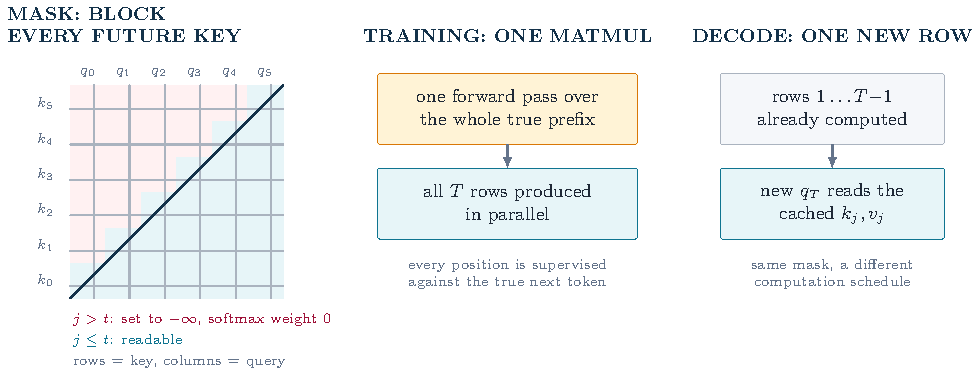
\includegraphics[width=\textwidth]{causal_mask.pdf}
\caption{因果自注意力的可见性与两种计算顺序。左：纵轴是 key 位置 \(k_j\)，横轴是 query 位置 \(q_t\)；对角线左上方 \(j>t\) 的格子设为 \(-\infty\)，softmax 权重为零。中：训练时一次前向并行算出注意力矩阵的全部 \(T\) 行（每个 query 一行）。右：解码时只有新的 \(q_T\) 读取缓存的 K/V；两者使用同一个 mask，只是计算顺序不同。}
\label{fig:causal-mask}
\end{figure}

\Needspace{10\baselineskip}
\section{注意力的几种变体：共享键值与汇总历史}

这里的“位置”是 token 在序列中的索引：\(t\) 表示当前要计算输出的 token，\(s\leq t\) 表示因果注意力可读取的第 \(s\) 个 token，其中 \(s<t\) 是先前 token，\(s=t\) 是当前 token。键 \(k_{s,i}\) 和值 \(v_{s,i}\) 由第 \(s\) 个 token 在本层的输入表示投影得到。前面的 MHA 有 \(h\) 个 query heads，每个 head 都用自己的 \(W_{Q,i},W_{K,i},W_{V,i}\) 投影，因此每个可见 token \(s\) 都为各 head 提供一组 \(k_{s,i},v_{s,i}\)。所谓\textbf{共享 K/V}，指多个 query heads 使用同一组 K/V 投影，读取同一个 token 时共用它的键和值；不同 token 的 K/V 仍然不同，query 投影也仍然按 head 区分。设第 \(i\) 个 query head 被分配到第 \(g(i)\) 组 K/V，其输出可以统一写成
\begin{equation}
 o_{t,i}=\sum_{s\le t}
 \frac{\exp\bigl(q_{t,i}^{\mathsf T}k_{s,g(i)}/\sqrt{d_k}\bigr)}
 {\sum_{r\le t}\exp\bigl(q_{t,i}^{\mathsf T}k_{r,g(i)}/\sqrt{d_k}\bigr)}
 v_{s,g(i)}.
\end{equation}
MHA 有 \(h\) 组 K/V，且 \(g(i)=i\)；多查询注意力（Multi-Query Attention，MQA）只有一组 K/V，所有 \(g(i)=1\)~\cite{shazeer2019mqa}；分组查询注意力（Grouped-Query Attention，GQA）保留介于两者之间的若干组，每组供多个 query heads 使用~\cite{ainslie2023gqa}。例如 8 个 query heads 配 2 组 K/V 时，每 4 个 query heads 共用一组 K/V 投影及其缓存。它们的 query 不同，所以即使读取同一组 K/V，softmax 权重和输出仍可不同。若有 \(n_{kv}\) 组 K/V，且各组维度相同，长度为 \(T\) 的已处理前缀需要保存约 \(Tn_{kv}(d_k+d_v)\) 个 K/V 数值；MQA 保存最少，GQA 居中，MHA 保留最多的 head 专属键值。共享减少了 K/V 缓存和生成时的读取量，也减少 K/V 投影参数，但 \(h\) 个 query heads 仍各自计算匹配权重，且共享越多，可供各 head 独立表达的前缀内容越少。

多头潜变量注意力（Multi-head Latent Attention，MLA）先把前缀中每个 token 的本层表示压成一个共享的低维向量，再由它生成各 head 所需的内容键和值，并另行处理位置相关信息~\cite{deepseekv2}。因此 MQA/GQA 是“多头共用几组键值”，MLA 是“每个 token 先存一份压缩表示，再供多头读取”；两者都保留按可见 token 做内容匹配和因果 mask。

\Needspace{7\baselineskip}
\textbf{局部窗口与少量全局 token。}另一种节省匹配次数的方式是稀疏注意力：普通 token 只读取邻近窗口及少量指定的全局 token，而全局 token 从较大范围读取并转递信息。Longformer 和 BigBird 用过这类结构处理长文档~\cite{beltagy2020longformer,zaheer2020bigbird}。其中“全局 token”是序列中的少数特殊 token；在自回归解码器中，它们的读写同样要遵守因果可见性，避免读到未来。另有局部层与全局层交替的做法：局部层只看滑动窗口，全局层让每个 token 查看完整可见前缀。这里的“全局”修饰整层的注意力范围，无需额外插入特殊 token。

\textbf{线性注意力：从 softmax 到递推状态。}先看一个注意力 head 在因果前缀上的输出。略去位置编码，普通 softmax 注意力可以写成
\begin{equation}
o_t^{\mathrm{softmax}}=
\frac{\sum_{s\le t}\exp\!\bigl(q_t^{\mathsf T}k_s/\sqrt{d_k}\bigr)v_s}
{\sum_{s\le t}\exp\!\bigl(q_t^{\mathsf T}k_s/\sqrt{d_k}\bigr)}.
\label{eq:softmax-causal-sum}
\end{equation}
每个历史位置的 value \(v_s\) 都按当前 query 与该位置 key 的匹配程度加权。新 query 到来时，分子和分母通常都要再次读取可见历史。

线性注意力保留“匹配后加权求和”这件事，但把指数匹配换成可拆开的非负内积~\cite{katharopoulos2020linear}。取固定维度 \(m\) 的特征映射 \(\phi:\R^{d_k}\to\R_{\geq0}^{m}\)，定义 \(a(q,k)=\phi(q)^{\mathsf T}\phi(k)\)。\(\phi\) 是对 query 和 key 的变换，例如逐元素使用指数线性单元（Exponential Linear Unit，ELU）构造 \(\operatorname{ELU}(x)+1\)；它不作用于 value。若 query 和 key 本来非负、\(\phi\) 取恒等映射，匹配权重就退化成 \(q^{\mathsf T}k\)。一般的 query 和 key 可以含负分量，直接去掉 softmax 而沿用原始点积会产生负权重或接近零的归一化分母；非负特征映射避免了这个问题，但新的权重通常不等于原来的 softmax 权重。

以这种基础形式为例，\(v_s\in\R^{d_v}\)。由于 \(\phi(q_t)\) 对求和中的每个历史位置都相同，可以把它移到求和外：
\begin{align}
o_t
&=\frac{\sum_{s\le t}\bigl[\phi(q_t)^{\mathsf T}\phi(k_s)\bigr]v_s}
{\sum_{s\le t}\phi(q_t)^{\mathsf T}\phi(k_s)+\varepsilon}
\label{eq:linear-attention-weighted}\\
&=\frac{\bigl(\sum_{s\le t}v_s\phi(k_s)^{\mathsf T}\bigr)\phi(q_t)}
{\bigl(\sum_{s\le t}\phi(k_s)\bigr)^{\mathsf T}\phi(q_t)+\varepsilon},
\qquad \varepsilon>0.
\label{eq:linear-attention-factored}
\end{align}
这里每个历史 token 对汇总状态贡献一项 \(v_s\phi(k_s)^{\mathsf T}\)：value 与变换后的 key 的外积。若 \(\phi\) 是恒等映射，它就是直观的 \(v_sk_s^{\mathsf T}\)；写出 \(\phi\) 是为了说明实际累加的是所选特征空间中的键值关联。

把上式两个与当前 query 无关的求和分别记为 \(S_t\) 和 \(z_t\)。新 token 到来时，只需在已有状态上增加它的一项，再用当前 query 读取：
\begin{align}
S_t&=S_{t-1}+v_t\phi(k_t)^{\mathsf T},\qquad S_0=0,\label{eq:linear-attention-state}\\
z_t&=z_{t-1}+\phi(k_t),\qquad z_0=0,\label{eq:linear-attention-normalizer}\\
o_t&=\frac{S_t\phi(q_t)}{z_t^{\mathsf T}\phi(q_t)+\varepsilon}.\label{eq:linear-attention-output}
\end{align}
\(S_t\in\R^{d_v\times m}\) 把 key 特征与 value 关联起来，\(z_t\in\R^m\) 保存归一化所需的特征总量。这里先把当前 \(k_t,v_t\) 写入状态，再用 \(q_t\) 读取，所以输出只依赖前 \(t\) 个 token（图 \ref{fig:linear-attention-state}）。

\begin{figure}[H]
\centering
\begin{tikzpicture}[node distance=12mm]
  \node[softblock,minimum width=27mm,minimum height=10mm] (past) {新 token\\\((k_t,v_t)\)};
  \node[tealblock,right=of past,minimum width=34mm,minimum height=10mm] (state) {固定大小的状态\\\(S_t,z_t\)};
  \node[softblock,right=of state,minimum width=23mm,minimum height=10mm] (read) {按查询读取};
  \node[softblock,right=of read,minimum width=17mm,minimum height=10mm] (out) {输出 \(o_t\)};
  \node[softblock,below=5mm of read,minimum width=23mm,minimum height=9mm] (query) {当前 \(\phi(q_t)\)};
  \draw[flow] (past) -- node[above,font=\scriptsize] {外积累加} (state);
  \draw[flow] (state) -- (read);
  \draw[flow] (query) -- (read);
  \draw[flow] (read) -- (out);
\end{tikzpicture}
\caption{每个新 token 把键值关联写入 \(S_t\)，当前 query 再从这份固定大小的状态读取。}
\label{fig:linear-attention-state}
\end{figure}

把 \(S_t\phi(q_t)\) 展开，就得到 \(\sum_{s\le t}v_s[\phi(k_s)^{\mathsf T}\phi(q_t)]\)。方括号中的内积衡量当前 query 与历史 key 在特征空间中的重合程度；重合越大，对应 value 在读出结果中的权重越大。\(z_t^{\mathsf T}\phi(q_t)\) 则汇总这些权重以完成归一化。因此 \(S_t\) 记住的是 key 与 value 的关联；多个 key 同时匹配时，读出的是相关 value 的加权混合。

当 \(m,d_v\) 固定时，更新和读取 \(S_t,z_t\) 的每步代价不随前缀长度增加，整段长度为 \(T\) 的序列所需的注意力计算随 \(T\) 线性增长。代价是多个 token 的键值关系合并在固定大小的状态中，不能像普通 softmax 注意力那样逐个寻址历史位置。

\Needspace{5\baselineskip}
从公开的自回归大模型看，保留可逐 token 寻址的 softmax 注意力及其窗口、GQA/MLA 或局部/全局层组合，仍比纯固定状态的线性注意力更常见：Mistral 7B 使用 GQA 与滑动窗口，Gemma 3 每五个局部注意力层配置一个全局注意力层~\cite{jiang2023mistral,gemmateam2025gemma3}。线性状态与可寻址注意力的混合也在发展，后文的 Kimi Linear 把 Kimi Delta Attention（KDA）层和 MLA 层交错使用~\cite{kimilinear}。

\begin{table}[H]
\centering\small
\begin{tabularx}{\textwidth}{>{\bfseries}p{28mm} X X}
\toprule
形式 & 历史信息怎样提供给 query & 主要取舍\\
\midrule
MHA & \(h\) 个 query heads 各有一组 K/V & 保留最多的 head 专属历史表示\\
MQA & \(h\) 个 query heads 共用一组 K/V & 历史存储最少，K/V 差异也最少\\
GQA & \(h\) 个 query heads 按组共用 K/V & 存储量与 K/V 多样性介于两者之间\\
MLA & 每个前缀 token 存低维向量，供各 head 生成 K/V & 压缩每个 token 的表示，增加投影步骤\\
局部窗口 + 全局 token & 普通 token 读窗口及少量全局 token & 保留稀疏的远程通道；因果生成需约束全局 token 的可见范围\\
局部层 + 全局层 & 局部层读窗口，全局层读完整可见前缀 & 保留按 token 寻址；全局层计算较重\\
线性注意力 & query 读取递推得到的 \(S_t,z_t\) & 状态大小固定，不能逐个寻址前缀 token\\
\bottomrule
\end{tabularx}
\caption{几种注意力形式的区别在于 query 能读取怎样的历史表示。}
\label{tab:attention-variants}
\end{table}

\section{Transformer 层的组件与词表输出}

\subsection{位置编码：绝对位置、RoPE 与 ALiBi}
\label{sec:rope}

位置编码解决的是自注意力本身对 token 排列置换不敏感的问题。绝对位置嵌入直接把一个可学习向量 \(p_t\) 加到 token 嵌入；它在训练长度内简单有效，但长度外推时没有未见过的位置向量。Rotary Position Embedding（RoPE）把每两维组成二维平面，在位置 \(m\) 施加旋转矩阵 \(R_{\theta,m}\)：
\begin{equation}
 q_m'=R_{\theta,m}q_m,\qquad k_n'=R_{\theta,n}k_n,\qquad
 (q_m')^\mathsf T k_n'
 =q_m^\mathsf T R_{\theta,n-m}k_n.
\end{equation}
最后一个等式说明内积依赖相对位置 \(n-m\)，这个依赖直接来自旋转角度的差。Attention with Linear Biases（ALiBi）保留 Q/K 原样，在 logit 中加入距离惩罚 \(b_h(m-n)\)~\cite{su2021rope,press2022alibi}。RoPE 的优势是保留多维相位关系，ALiBi 的优势是形式简单、距离偏置直接；两者都需要与训练长度、频率尺度和数值范围一起设计。

\subsection{归一化与残差连接}

层归一化（Layer Normalization，LayerNorm）对每个 token 的 \(d\) 维向量单独计算通道均值和方差，再把各通道的数值调整到稳定尺度，不在不同 token 之间求统计量。对 \(x\in\R^d\)，令 \(\mu(x)=d^{-1}\sum_jx_j\)、\(s^2(x)=d^{-1}\sum_j[x_j-\mu(x)]^2\)，则
\begin{equation}
 \operatorname{LayerNorm}(x)_j=\gamma_j\frac{x_j-\mu(x)}{\sqrt{s^2(x)+\varepsilon}}+\beta_j.
\end{equation}
其中 \(\varepsilon\) 是防止分母过小的固定常数；\(\gamma,\beta\in\R^d\) 分别是训练得到的逐通道缩放和偏移，每个 LayerNorm 层有 \(2d\) 个可训练参数。均值和方差由当前输入计算；同一层的 \(\gamma,\beta\) 在所有 token 位置共享。

对注意力或 FFN 子层 \(\mathcal F_l\)，Post-Norm 在残差相加后归一化，即 \(h_{l+1}=\operatorname{Norm}(h_l+\mathcal F_l(h_l))\)。Pre-Norm 先归一化子层输入，再把输出加回原始残差，即 \(h_{l+1}=h_l+\mathcal F_l(\operatorname{Norm}(h_l))\)。两者使用相同的归一化规则，差别在归一化的位置；图 \ref{fig:transformer-block} 左侧是一个 Pre-Norm block。Pre-Norm 给梯度提供更直接的残差路径，深层训练通常更稳定；均方根归一化（Root Mean Square Layer Normalization，RMSNorm）只用
\begin{equation}
\operatorname{RMSNorm}(x)_j=\gamma_j\frac{x_j}{\sqrt{d^{-1}\sum_kx_k^2+\varepsilon}},
\end{equation}
省去减去均值和可训练的偏移 \(\beta\)，每层仅保留 \(d\) 个缩放参数，相应减少计算和参数~\cite{zhang2019rmsnorm}。归一化在概率模型中承担的是尺度控制：让矩阵乘法、softmax 和残差叠加中的数值范围保持稳定。

\subsection{前馈网络：非线性与门控}

注意力负责位置之间的信息交换，FFN 负责把每个位置已收集的信息组合成新特征。若只堆叠线性映射，多层仍等价于一个线性映射；在升维与降维之间加入非线性，才能表达更复杂的特征组合。基本 FFN 为
\begin{equation}
 \operatorname{FFN}(h)=W_2\,\varphi(W_1h+b_1)+b_2,
\end{equation}
其中 \(d_{\mathrm{ff}}\) 是中间宽度，\(\varphi\) 是逐元素激活函数。高斯误差线性单元（Gaussian Error Linear Unit，GELU）的精确定义是 \(\varphi(x)=x\Phi(x)\)，其中 \(\Phi\) 是标准正态分布的累积分布函数；BERT 和视觉 Transformer 的前馈层都使用 GELU~\cite{devlin2019bert,dosovitskiy2021vit}。

现代模型中常用 sigmoid 线性单元（Sigmoid Linear Unit，SiLU）。它的具体函数是
\begin{equation}
 \sigma(x)=\frac{1}{1+e^{-x}},\qquad
 \operatorname{SiLU}(x)=x\sigma(x)=\frac{x}{1+e^{-x}}.
 \label{eq:silu}
\end{equation}
这里 \(\sigma\) 是 sigmoid 函数。SiLU 将输入乘以一个介于 0 和 1 之间的平滑系数：较大的正输入近似保留，较大的负输入趋于零，靠近零的负输入仍可通过。它在全域可微，且 \(\operatorname{SiLU}'(0)=1/2\)，所以零附近仍有梯度；通常所说的 Swish 在门控尺度取 1 时就是 SiLU。

单个激活函数只变换一个分支。门控线性单元（Gated Linear Unit，GLU）进一步使用两条投影：一条提供内容，另一条根据输入控制各通道的系数。SwiGLU（Swish Gated Linear Unit，Swish 门控线性单元）用 SiLU 处理门控分支~\cite{shazeer2020glu}：
\begin{equation}
 g=W_gh,\qquad u=W_uh,\qquad
 \operatorname{SwiGLU}(h)=W_d[\operatorname{SiLU}(g)\odot u].
 \label{eq:swiglu}
\end{equation}
\(W_g,W_u\) 将表示升到中间宽度，\(\odot\) 表示对应通道逐元素相乘，\(W_d\) 再投影回残差维度。门控让同一内容分支在不同输入下有不同的通道权重；门控分支的输出 \(\operatorname{SiLU}(g)\) 可以为负，也不限于 \([0,1]\)，因此它提供连续的可学习调制。训练梯度同时更新两个升维分支和降维矩阵。

\begin{figure}[ht]
\centering
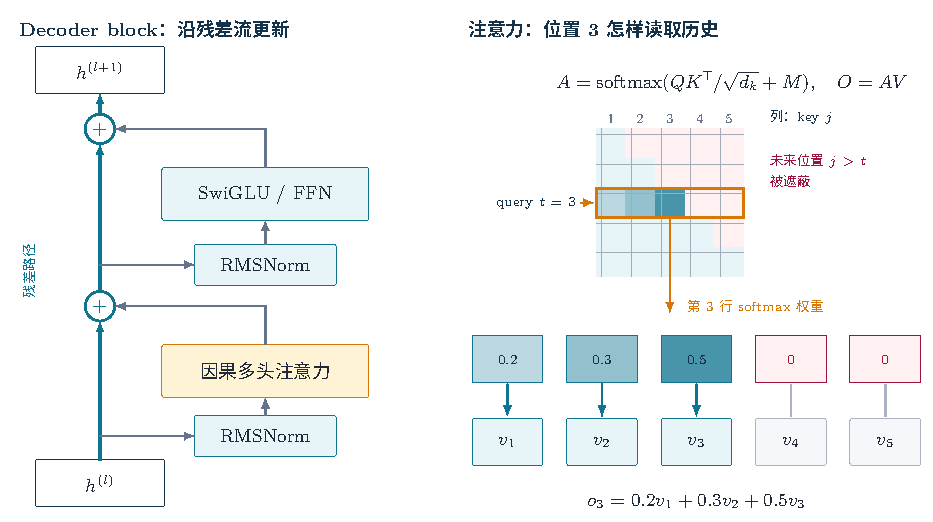
\includegraphics[width=\textwidth]{transformer_block_detailed.pdf}
\caption{一个 Pre-Norm decoder block 与一次因果注意力读取。左侧两条子层分支都从残差流取输入，计算后再加回；词表投影发生在堆叠的 block 之后。右侧以位置 3 为例：遮蔽未来位置，取注意力矩阵的第 3 行；等宽色块中的数字是示意权重，只有前三个 value 参与输出。}
\label{fig:transformer-block}
\end{figure}

\subsection{词表输出与训练、生成流程}

最后一个 block 的隐藏状态还不直接是概率。若位置 \(t\) 输入的是 \(x_t\)，那么 \(h_t^{(L)}\) 已经读取 \(x_{\le t}\)，用于预测 \(x_{t+1}\)；BOS 对应位置 \(t=0\)。模型先算出词表 logits
\begin{equation}
 l_t=W_{\mathrm{vocab}}h_t^{(L)}\in\R^{|\mathcal V|},
 \qquad
 p_\theta(x_{t+1}=v\mid x_{\le t})=\frac{\exp(l_{t,v}/\tau)}{\sum_{u\in\mathcal V}\exp(l_{t,u}/\tau)},
\end{equation}
其中 \(W_{\mathrm{vocab}}\in\R^{|\mathcal V|\times d}\) 是词表投影，往往与输入嵌入共享参数；\(\tau\) 在这里是采样温度，训练时取 \(\tau=1\)，此时这一行就是一个标准 softmax。所以“残差流中的向量”到“下一个 token 的概率”之间只有一次线性投影加一次 softmax，整个模型的输出维度就是词表大小 \(|\mathcal V|\)。

对一个长度为 \(T\) 的 batch，训练时把真实 token 序列一次送入网络；causal mask 使第 \(t\) 行只能使用 \(1,\ldots,t\) 的表示，各位置仍可并行计算。每个位置产生 logits \(l_t\)，softmax 给出词表分布，交叉熵取出真实下一个 token 的负对数概率，梯度再经过词表投影、FFN、注意力和输入嵌入传播。生成时把新 token 加入前缀，再计算下一个位置的条件分布；新的位置必须等待上一步的输出。

\section{解码：从 logits 到文本}
\label{sec:decoding}

模型给出的是每个位置上的条件分布 \(p_\theta(\cdot\mid x_{<t})\)；解码要做的是从中选一个 token，再把它接回前缀。选择方式会改变整条序列的分布，也会改变生成结果的多样性、重复程度和可复现性。下面按“是否保持模型分布”把常用做法分成几组。

\textbf{确定性与搜索。}贪心解码每一步取概率最大的 token。它可复现、延迟最低，代价是容易陷入重复循环，生成结果偏离 \(p_\theta\) 的联合分布。beam search 保留 \(B\) 条累计对数概率最高的部分序列，在每一步扩展后重新排序，最后取分数最高的一条。它近似寻找 \(p_\theta\) 下概率最高的序列，即分布的众数，结果是确定的，不对应 \(p_\theta\) 的随机样本；beam 越大，结果越保守，越容易偏向训练数据里常见的表达。对比解码（contrastive decoding）用一大一小两个模型的对数概率之差给 token 打分，压低小模型也会给高概率的通用、模板化 token~\cite{li2023contrastive}；DoLa（Decoding by Contrasting Layers）在同一模型内做类似比较，用深层与浅层输出的对数概率之差~\cite{chuang2023dola}。

\textbf{随机采样。}温度采样把 logit 除以 \(\tau\) 再做 softmax：\(\tau<1\) 使分布更尖，\(\tau>1\) 使分布更平。top-\(k\) 只保留概率最高的 \(k\) 个 token 后重新归一化；nucleus sampling（top-\(p\)）保留累计概率首次达到 \(p\) 的最小集合~\cite{holtzman2020curious}；min-\(p\) 保留概率不低于最大概率固定比例的 token；locally typical sampling 保留那些“信息量接近当前分布熵”的 token~\cite{meister2022typical}。这些操作都在改变分布：只有不截断且 \(\tau=1\) 时，逐步随机抽取才严格对应模型自身的 \(p_\theta(x)\)。

\textbf{惩罚项。}repetition penalty 对已经出现过的 token 降低 logit；frequency 和 presence penalty 按出现次数或是否出现来调整；no-repeat n-gram 直接禁止重复的 \(n\) 元组。它们都在 logits 上做加法或除法，因此同样改变分布。惩罚过强时，模型会回避必要的重复，例如化学式里的下标或代码里的括号，需要按任务调。

\textbf{约束解码。}如果输出必须符合某种结构，可以在每一步把不合法的 token 概率置零：正则表达式、JSON schema、语法都能编译成有限状态机，解码器只保留仍能走到合法终止状态的 token。这样得到的输出一定合法，但分布被限制在一个子集上，语言质量可能下降；约束越复杂，每步的掩码检查越贵。

\textbf{多采样与验证。}对同一问题独立生成多条回答，再用多数投票（self-consistency）或一个验证器挑选，属于推理时的额外计算~\cite{wang2023selfconsistency}。它改变的是最终交付的答案，模型分布保持不变；第 \ref{sec:test-time-scaling} 节的推理式扩展会回到这一点。

把上面几组放在一起，可以看出解码是“模型分布”与“任务约束”相遇的地方。表 \ref{tab:decoding-ops} 按“是否保持 \(p_\theta\)”归纳。

\begin{table}[H]
\centering\small
\begin{tabularx}{\textwidth}{>{\bfseries}p{40mm} p{30mm} X X}
\toprule
操作 & 改变发生在哪一步 & 作用 & 代价\\
\midrule
按模型分布采样（\(\tau=1\)、不截断） & 无，严格对应 \(p_\theta\) & 得到模型自身的样本 & 长尾与重复不受控\\
贪心 / beam search & 选择规则：退化为点估计或近似最大后验 & 稳定、可复现 & 容易重复、缺乏多样性；beam 计算量随宽度增加\\
温度、top-\(k\)、top-\(p\)、min-\(p\)、typical & 采样分布：平滑、截断或重归一化 & 控制多样性与生成长度 & 困惑度与校准不再对应 \(p_\theta\)\\
重复惩罚 & logit & 抑制循环 & 可能压掉必要的重复\\
约束解码 & 支撑集：限制在合法序列 & 保证输出符合语法或 schema & 质量可能下降\\
self-consistency / best-of-\(N\) & 最终答案的选择 & 提高最终答案的正确率 & 多次生成与评分\\
\bottomrule
\end{tabularx}
\caption{解码操作对分布的影响：只有不截断、\(\tau=1\) 的按分布采样保持 \(p_\theta\)；其余做法分别在选择规则、采样分布、logit、支撑集或最终答案上改变结果。}
\label{tab:decoding-ops}
\end{table}

\section{专家混合（Mixture of Experts，MoE）：把 FFN 换成稀疏路由}
\label{sec:moe}

普通 FFN 的所有参数都会对每个 token 执行计算。MoE 把这一子层换成多组独立的 FFN，称为专家，再让每个 token 只经过其中的 \(k\) 组~\cite{shazeer2017moe}。Switch Transformer 是每个 token 只选一个专家（\(k=1\)）的例子~\cite{fedus2022switch}。若有 \(N_{\mathrm{exp}}\) 个专家且 \(k\ll N_{\mathrm{exp}}\)，模型可以增加可选的参数总量，而单个 token 只执行选中专家的计算；注意力和残差路径仍按前面的方式工作。

\subsection{路由与容量}

路由器（router）读取当前位置表示 \(h_t\)，给每个专家一个分数并选出最高的 \(k\) 个：
\begin{equation}
 p_t=\operatorname{softmax}(W_rh_t),\qquad
 \mathcal S_t=\operatorname{TopK}(p_t,k),\qquad
 y_t=\sum_{e\in\mathcal S_t}\widetilde p_{t,e}\operatorname{FFN}_e(h_t).
\end{equation}
其中 \(W_r\in\R^{N_{\mathrm{exp}}\times d}\) 是可训练的路由矩阵，\(\widetilde p_{t,e}=p_{t,e}/\sum_{j\in\mathcal S_t}p_{t,j}\) 是选中专家之间的归一化权重。位置 \(t\) 的输出由这些专家的结果加权组合，再像普通 FFN 输出一样进入残差连接。

\(\operatorname{TopK}\) 决定“选谁”，这个离散选择本身不提供普通的连续梯度；在选中集合确定时，损失仍能通过 \(\widetilde p_{t,e}\) 更新路由器，并更新被选中专家的参数。未被选中的专家不会从该 token 得到主损失梯度。

实际执行还要给每个专家设一个容量上限。若一个 batch 有 \(B\) 个 token、\(N_{\mathrm{exp}}\) 个专家，容量常写成
\begin{equation}
 C=\text{capacity factor}\times\frac{B}{N_{\mathrm{exp}}},
\end{equation}
超出的 token 被丢弃，或者绕过专家直接沿残差路径通过。容量因子大于 1 留出余量，代价是显存和通信按容量预留；小于 1 则主动丢弃，吞吐稳定但质量下降。训练时可以用辅助损失让负载均匀，Switch Transformer 的形式是
\begin{equation}
 \mathcal L_{\mathrm{aux}}=N_{\mathrm{exp}}\sum_{e=1}^{N_{\mathrm{exp}}}f_eP_e,
 \label{eq:moe-aux}
\end{equation}
其中 \(f_e\) 是分给专家 \(e\) 的 token 比例，\(P_e\) 是该专家收到的平均路由概率~\cite{fedus2022switch}。它鼓励两者都接近 \(1/N_{\mathrm{exp}}\)。辅助损失与语言模型损失一起下降，系数太大会牺牲专家的专门化；DeepSeek-V3 改用一组按负载统计直接调整的选择偏置，不进入梯度，第 \ref{chap:modern-arch} 章会看到具体做法。

\subsection{共享专家与细粒度专家}

基础 MoE 让每个 token 在若干完整 FFN 之间选择。两种改动可以减少路由的浪费。一是把专家划得更细：用更多、更小的 FFN，每个 token 选更多个，组合数增加，而总计算量仍由 \(k\) 控制。二是保留一个所有 token 都经过的共享专家，让它承接各任务共有的变换，路由专家只负责差异部分~\cite{deepseekv2}。共享专家增加固定计算，但减少了路由专家需要重复学习的内容。

细粒度与共享专家一起用时，常见配置是“一个共享专家加多个细粒度路由专家”，每个 token 选其中少数几个。专家总数可以远大于单个 token 实际执行的专家数，参数量随之增加，但每 token 的浮点运算量仍接近一个稠密 FFN 的若干倍。

\subsection{专家并行与通信}

专家数量超过单卡容量后，不同专家被放到不同设备上，这就是专家并行（Expert Parallelism，EP）。路由器决定每个 token 去哪些设备，执行前把表示发送过去（dispatch），执行后把结果送回原位置（combine），两次都是 all-to-all 通信。若每个 token 选 \(k\) 个专家、表示宽度为 \(d\)、每个元素 \(b\) 字节，那么一个 token 往返的通信量约为 \(2kbd\) 字节；一个 batch 的总量再乘 token 数。

这条估算解释了后面几种设计。容量因子限制了单个设备一次要接收多少 token，负载不均会让某些设备成为等待的瓶颈；把路由分支压到低维潜空间（第 \ref{chap:modern-arch} 章的 Stable LatentMoE）相当于把上式中的 \(d\) 换成更小的 \(\ell\)；共享专家不经过路由，因此不产生跨设备流量。EP 通常与数据并行、张量并行和流水线并行组合使用，第 \ref{chap:training-stability} 章的多卡训练会把这些轴放在一起。
